\documentclass[naustrian]{article}
\usepackage[T1]{fontenc}
\usepackage[utf8]{inputenc}
\usepackage{cite}
\usepackage{geometry}
\geometry{verbose,tmargin=3cm,bmargin=3cm,lmargin=3cm,rmargin=3cm}
\usepackage[ngerman]{babel}
\usepackage{microtype}
\usepackage[parfill]{parskip}
\usepackage{amsmath}
\usepackage{graphicx}
\usepackage[unicode=true] {hyperref}
\usepackage{pdfpages}
\usepackage{float}
\usepackage{url}

\begin{document}

\title{Mehrdimensionale Optimierung ohne Nebenbedingungen}

\author{Sonja Biedermann, Felix Freynschlag, Bernhard Hayden,\\
Stepan Kharin, Christoph Pressler}

\maketitle
\tableofcontents
\listoffigures

\section{Das Nelder-Mead-Verfahren}

\subsection{Einführung}

Das Nelder-Mead-Verfahren (auch Downhill-Simplex genannt) verfolgt
einen geometrischen Ansatz zur iterativen Optimierung: ein Simplex
bestehend aus $N+1$ Punkten (im Falle $N=2$, dem zweidimensionalen
Raum, also ein Dreieck) wird fortwährend so transformiert, sodass
sich der Simplex dem Minimum nähert, um welches er sich dann zusammenzieht.\cite{nelder-mead-enwiki}

\subsection{Funktionsweise}

Der Algorithmus besteht im wesenstlichen aus drei
Phasen\cite{nelder-mead-scholarpedia}, die in jeder Iteration durchlaufen
werden:
\begin{enumerate}
    \item Ordering
    \item Centroid
    \item Transformation
\end{enumerate}

\paragraph{Ordering}

Zu Beginn besitzen wir $N+1$ Punkte, die anhand irgendwelche Kriterien
(durchaus auch zufällig) gewählt wurden. Diese müssen wir nun anhand
ihrer Güte ordnen, also sortieren. Im Falle des zweidimensionalen
Raumes erhalten wir also die drei mnemonisch benannten Punkte \textbf{$B$
}(\emph{best}), $G$ (\emph{good}) und $W$ (\emph{worst}).\cite{nelder-mead-unknown} $B$ ist
im Falle eine Minimierung der Punkt, dessen Funktionswert am geringsten
ist, $G$ der mit dem zweit geringsten Wert, und so weiter.


\paragraph{Centroid}

Als nächstes berechnen wir den Mittelpunkt der beiden besseren Punkte

\[
    M=\frac{B+G}{2}
\]
und nehmen diesen als Basis für unsere weiteren Berechnungen.


\paragraph{Transformation}

Nun reflektieren wir den schlechtesten Punkt $W$ am Mittelpunkt
\[
    R=M+\alpha(M-W)
\]
und prüfen, ob dieser Punkt $R$ die Relation $f(B)\leq f(R)\leq f(W)$
erfüllt.

Wenn ja, ersetzen wir den schlechtesten Punkt mit $R$ und brechen
die jetzige Iteration ab. Diesen Vorgang nennt man auch das ,,Akzeptieren``
eines Punktes.

Wenn nein, prüfen wir, ob der reflektierte Punkt $R$ besser als unser
bisher bester Punkt ist, also ob $f(R)<f(B)$ gilt. Wenn dem so ist,
expandieren wir den Punkt $R$ testweise weiter:
\[
    E=M+\gamma(M-W)
\]
und prüfen wiederum, ob dieser Punkt $E$ besser als unser reflektierte
Punkt $R$ ist. Wenn ja, akzeptieren wir $E$. Wenn nein, akzeptieren
wir $R$.

Gilt $f(R)\geq f(G)$, so ist der reflektierte Punkt kein guter Kandidat.  Wir
müssen nun die zwei möglichen kontrahierten
Punkte\cite{nelder-mead-scholarpedia} $C_{1}$, $C_{2}$
berechnen.\cite{nelder-mead-unknown} Gilt $f(R)<f(W)$, berechnen wir den
äußeren kontrahierten Punkt $C_{1}$, ansonsten den inneren kontrahierten Punkt
$C_{2}.$
\begin{eqnarray*}
    C_{1} & = & M+\rho(R-M)\\
    C_{2} & = & M+\rho(W-M)
\end{eqnarray*}

Sind die berechneten kontrahierten Punkte besser als die zur Berechnung
verwendeten Punkte ($R$ und $W$ respektive), so werden diese akzeptiert.
Ist dem nicht so, müssen wir zum nächsten Schritt, der Komprimierung,
fortfahren. Bei der Komprimierung werden jediglich die zwei schlechteren
Punkte $G$ und $W$ in Richtung des besten Punktes $B$ gezogen.
\begin{eqnarray*}
    G & = & B+\sigma(B-G)\\
    W & = & B+\sigma(B-W)
\end{eqnarray*}
\rule[0.5ex]{1\columnwidth}{1pt}\\

Diese Schritte werden fortgeführt, bis eine Abbruchbedingung eintritt,
wie etwa dass der Unterschied zwischen dem besten Funktionswert $f(B)$
und dem schlechtesten Funktionswert $f(W)$ oder der Umfang des Simplex' ein gegebenes $\varepsilon$
unterschreitet.

\subsection{Erläuterung der einzelnen Transformationsschritte}

Folgend werden die einzelnen Transformationsschritte anhand eines
Dreiecks als Simplex vorgeführt und erläutert. Für unsere Koeffizienten
wählen wir die Werte $\alpha=1,\,\gamma=2,\,\rho=\frac{1}{2},\,\sigma=\frac{1}{2}$.
Unser Dreieck $\triangle BGW$ ist definiert mit $B=(1,\,3),\,G=(4,\,6),\,W=(6,\,2)$.

\begin{figure}[H]
    \centering
    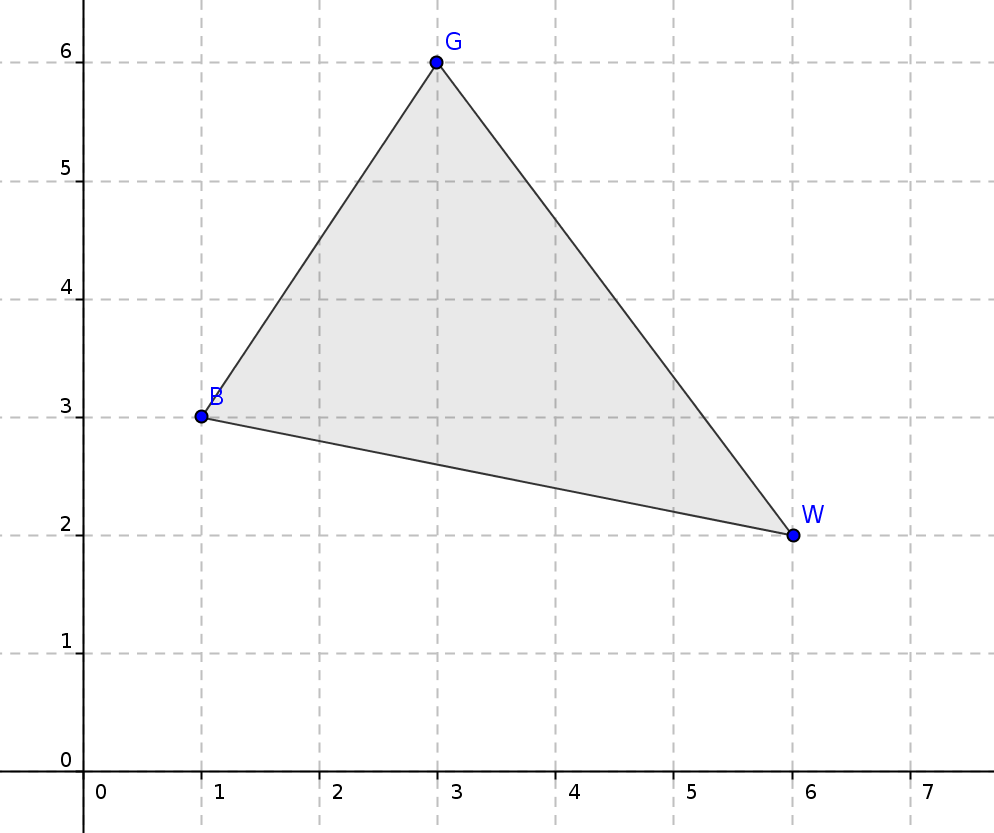
\includegraphics{nelder_mead/triangle_bgw}
    \caption{Unser Ursprungssimplex}
\end{figure}

\subsubsection{Reflektion}

Wir reflektieren den schlechtesten Punkt an dem Mittelpunkt in die
vermeintlich bessere Richtung.
\[
    R=M+M-W=2M-W=\binom{5}{9}-\binom{6}{2}=\binom{-1}{7}
\]

\begin{figure}[H]
    \centering
    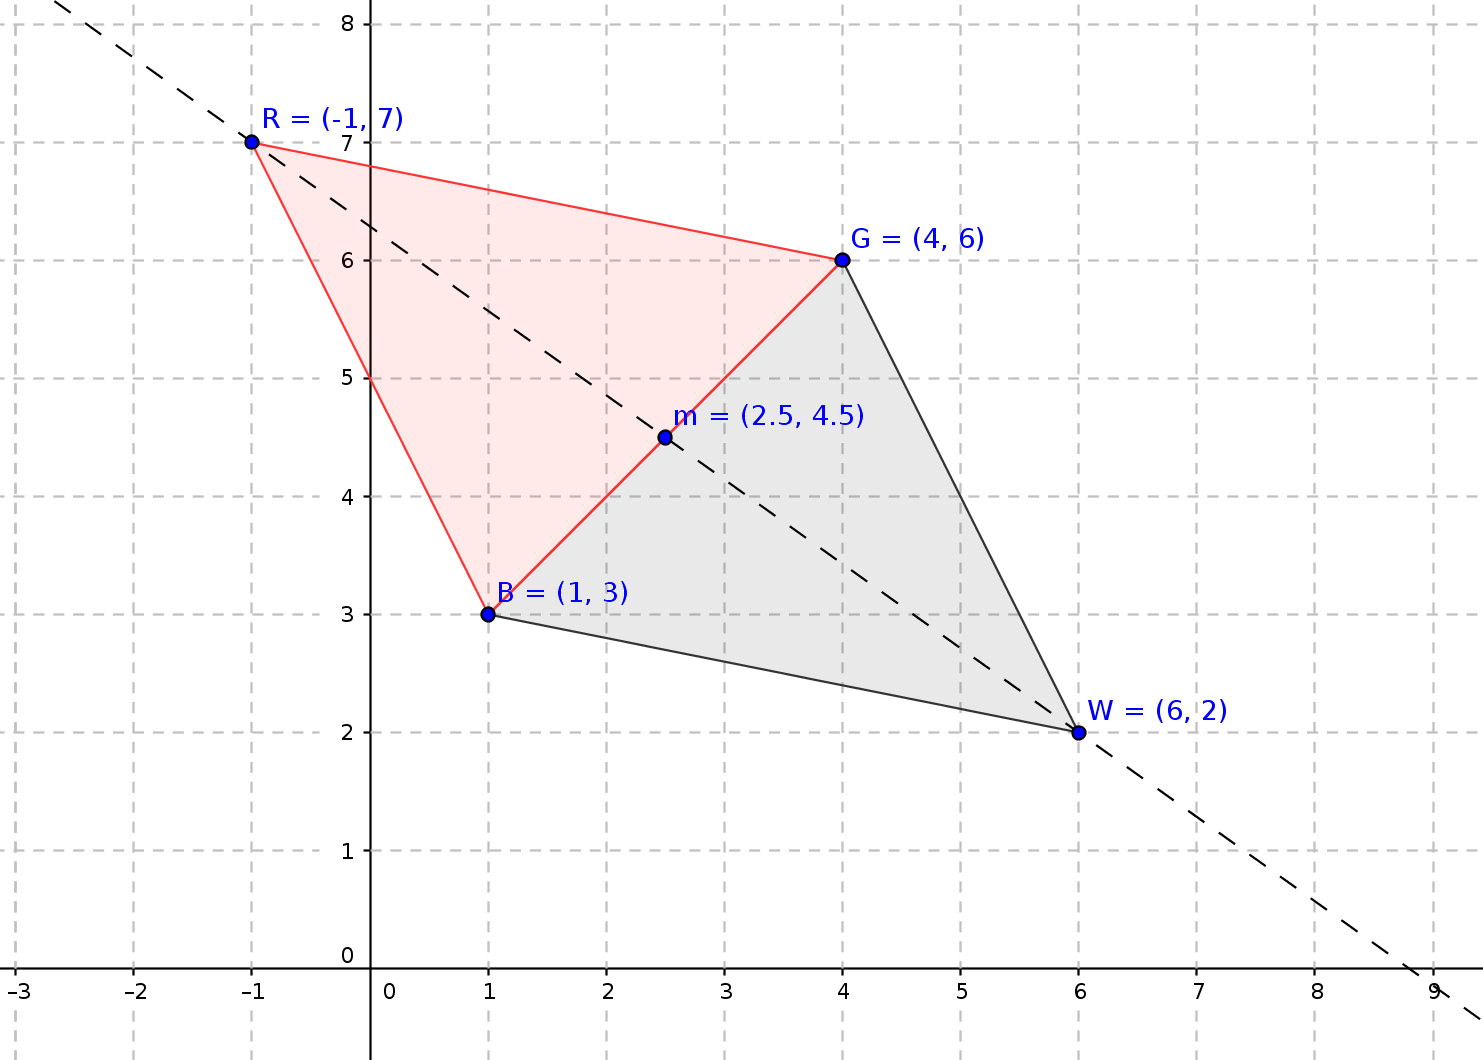
\includegraphics{nelder_mead/triangle_reflect}
    \caption{Nach der Reflektion}
\end{figure}

Dies entspricht dem ,,Heruntertaumeln`` des Simplex, welches die
Optimierung in den ersten Iterationsschritten unter anderem antreibt.

\subsubsection{Expansion}

Nehmen wir an, dass $f(R)$ besser als unser bis jetzt bester Wert
ist. Wir expandieren also weiter:

\[
    E=M+2(M-W)=\binom{2.5}{4.5}+\binom{-7}{5}=\binom{-4.5}{9.5}
\]

\begin{figure}[H]
    \centering
    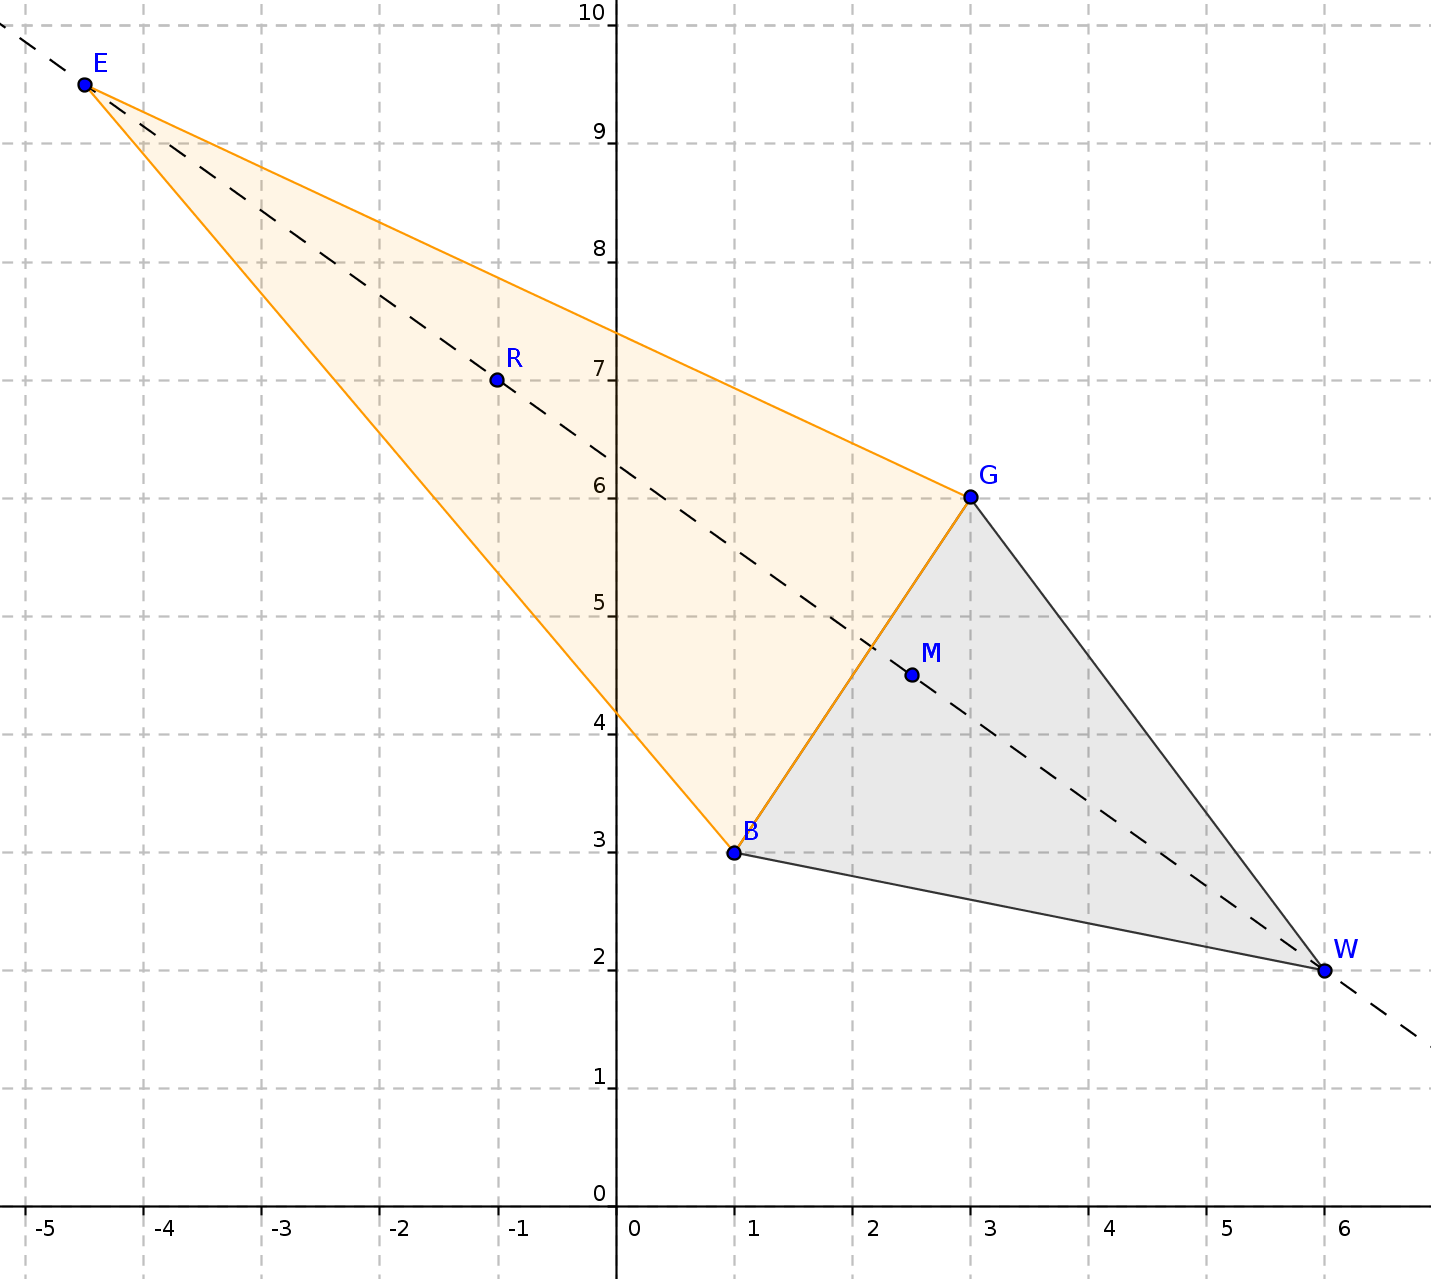
\includegraphics{nelder_mead/triangle_expand}
    \caption{Nach der Expansion}
\end{figure}

Dies entspricht einem {\emph{greedy approach} -- dieser
Schritt ist nicht notwendig per se, minimiert aber zusätzlich die Anzahl
der nötigen Iterationen. In schwer zu optimierenden Funktionen, wie etwa
Rosenbrock's Bananenfunktion, kann der Expansionsfaktor $\gamma$ dazu genutzt werden,
den Simplex in flachem Gelände schneller wandern zu lassen.

\subsubsection{Kontraktion}

Gehen wir jetzt vom Gegenteil aus \textendash{} Punkt $R$ war also
kein geeigneter Punkt und Punkt $E$ wurde gar nicht berechnet \textendash{}
so müssen wir die beiden Kontraktionspunkte $C_{1}$, $C_{2}$ berechnen.
\begin{eqnarray*}
    C_{1} & = & M+\frac{R-M}{2}=\binom{2.5}{4.5}+\frac{\binom{-1}{7}-\binom{2.5}{4.5}}{2}=\binom{-1.75}{1.25}\\
    C_{2} & = & M+\frac{W-M}{2}=\binom{2.5}{4.5}+\frac{\binom{6}{2}-\binom{2.5}{4.5}}{2}=\binom{4.25}{1.25}
\end{eqnarray*}

\begin{figure}[H]
    \centering
    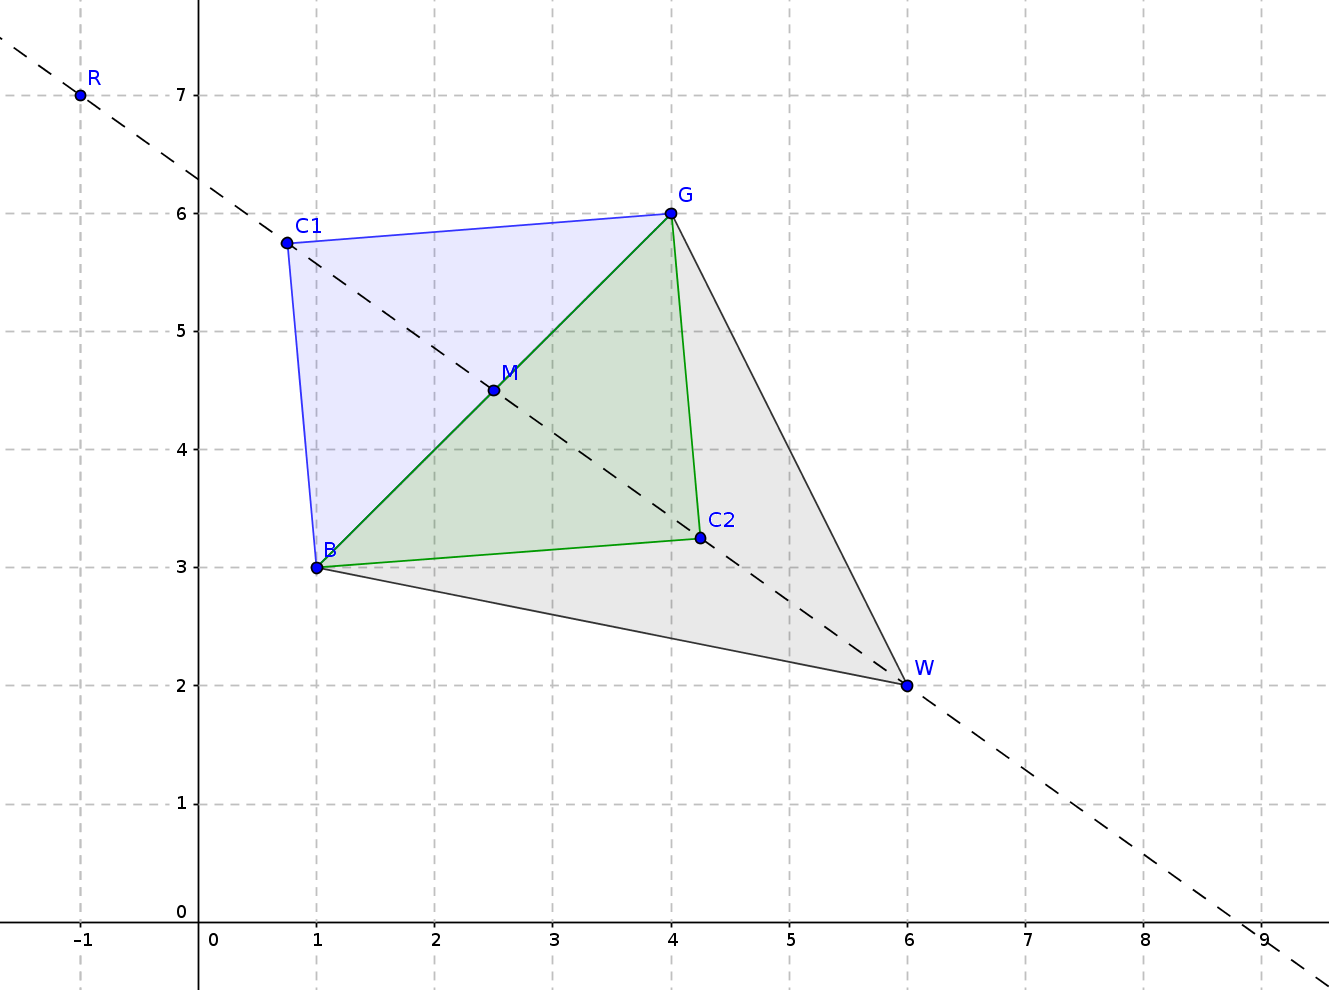
\includegraphics{nelder_mead/triangle_contract}
    \caption{Nach der Kontraktion}
\end{figure}

\subsubsection{Komprimierung}

Wir komprimieren die Punkte $G$ und $W$ in Richtung $B$.
\begin{eqnarray*}
    G' & = & B+\frac{G-B}{2}=\binom{1}{3}+\binom{1}{1.5}=\binom{2}{4.5}\\
    W' & = & B+\frac{W-B}{2}=\binom{1}{3}+\binom{2.5}{-0.5}=\binom{3.5}{2.5}
\end{eqnarray*}

\begin{figure}[H]
    \centering
    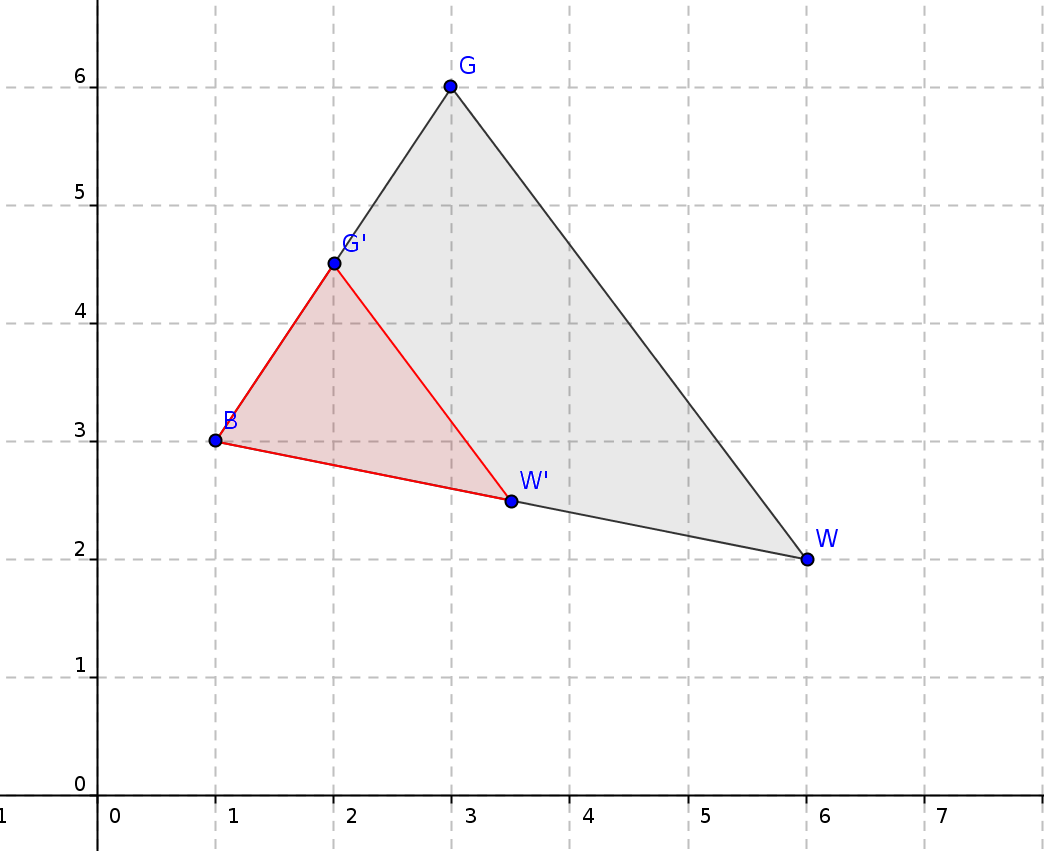
\includegraphics{nelder_mead/triangle_compress}
    \caption{Nach der Komprimierung Richtung $B$}
\end{figure}

Dies entspricht dem Zusammenziehen des Simplex' in den letzten Iterationsschritten
des Algorithmus'.


\subsection{Ein Beispiel: die Himmelblau-Funktion}

\begin{figure}[H]
    \centering
    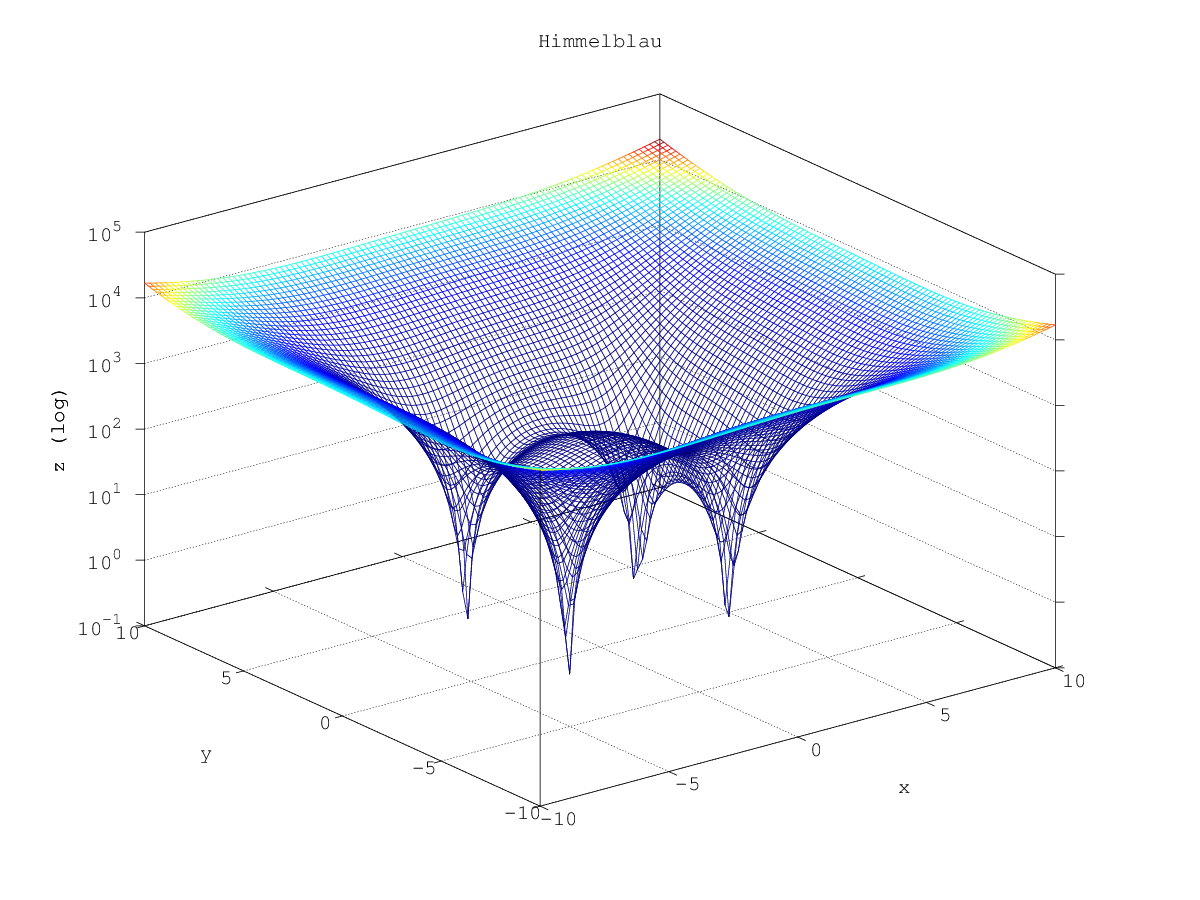
\includegraphics[width=0.7\textwidth]{nelder_mead/himmelblau}
    \caption{Die Himmelblau Funktion auf logarithmischer $z$-Skala}
\end{figure}

Um unseren Algorithmus exemplarisch vorzuführen, wollen wir die Himmeblau-
Funktion minimieren. Dazu verwenden wir die beiliegende {\tt C++}-Implementierung, um
die hier aufgelisteten Graphiken zu generieren.

Die Himmelblau-Funktion ist definiert als

\[
    f(x,y) = (x^2 + y - 11)^2 + (x + y^2 - 7)^2
\]

und hat 4 gleiche lokale Minima an den Stellen

\begin{eqnarray*}
    f(3.2, 2.0) & = & 0.0\\
    f(-2.805118, 3.131312) & = & 0.0\\
    f(-3.779310, -3.283186) & = & 0.0\\
    f(3.584428, -1.848126) & = & 0.0\\
\end{eqnarray*}

Wir wollen unseren Algorithmus auf sie loslassen, um eines davon zu finden. Als
Abbruchbedingung wählen wir

\[
    \Delta f_{W,B} \leq 0.1,
\]

also dass der Unterschied des besten und schlechtesten Funktionswert kleiner
gleich $0.1$ ist. Wir wählen diesen so groß, weil wir aus Platzgründen lieber
schnell konvergieren als ein möglichst genaues Resultat wollen.

Unsere Startpunkte sind folgende:
\begin{eqnarray*}
    P_{1} & = & (-1,\,-5)\\
    P_{2} & = & (3,\,-8)\\
    P_{3} & = & (8,\,8)
\end{eqnarray*}

Wie bereits besprochen, sind die Startpunkte relativ egal und wurden auch hier
recht zufällig gewählt. Die einzige Einschränkung des Startsimplex ist, dass es
sich hierbei auch um einen tatsächlichen Simplex handeln muss (ein
degenerierter Simplex wäre nutzlos). Weiters ist ein großer Simplex
wünschenswert, da gegebenenfalls zu Beginn einer Optimierung große Schritte in
Richtung Minimum gemacht werden müssen, um schnell konvergieren zu können. Ein
kleiner Simplex benötigt weit mehr Zeit um zu konvergieren -- dieses Problem
kann man beispielsweise bei Rosenbrock's Banenenfunktion beobachten, die in der
beiliegenden Implementierung ebenfalls vorhanden ist.

\begin{figure}[H]
    \centering
    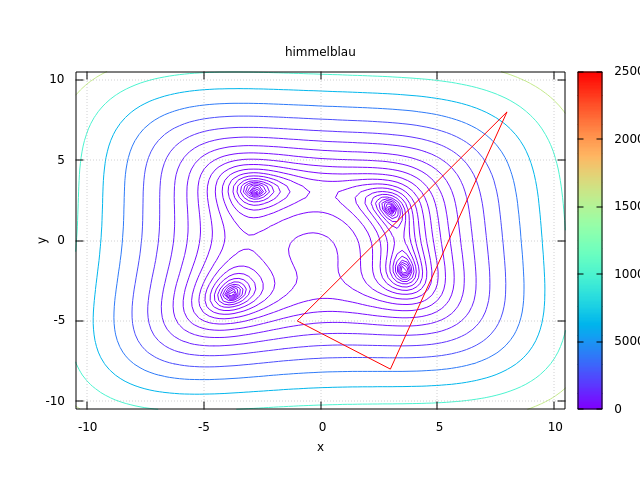
\includegraphics[width=0.7\textwidth]{nelder_mead/1}
    \caption{Unser Anfangssimplex aufgetragen auf einen Contourplot der Himmelblau-Funktion.}
\end{figure}

Der erste Schritt ist das Ordnen der Punkte nach ihrem Funktionswert. Wir berechnen:

\begin{eqnarray*}
    f(P_{1}) & = & 512\\
    f(P_{2}) & = & 3700\\
    f(P_{3}) & = & 7964
\end{eqnarray*}

Netterweise sind unsere Punkte also schon geordnet und $P_{1}$, $P_{2}$ und $P_{3}$ entsprechen jeweils
$B$, $G$, und $W$. Wir fahren fort und berechnen den Mittelpunkt

\[
    M = \frac{B + G}{2} = \binom{1}{-6.5}
\]

Als nächstes berechnen wir den reflektierten Punkt

\[
    R = 2M - W = \binom{-6}{-21}
\]

Berechnen wir nun $f(R) = 183200$, sehen wir, dass der reflektierte Punkt keine gute Idee ist. Da $R$
bei weitem schlechter als unser schlechteste Punkt $W$ ist, berechnen wir den inneren kontrahierten Punkt

\[
    C_{2} = M + \frac{W - M}{2} = \binom{4.5}{0.75}
\]

Berechnen wir nun $f(C_{2}) = 103.75391$, sehen wir, dass
wir einen guten Fortschritt gemacht haben. Wir ersetzen
$W$ und ordnen unsere Punkte neu.

\begin{eqnarray*}
    B & = & (4.5, \, 0.75)\\
    G & = & (-1,\,-5)\\
    W & = & (3,\,-8)
\end{eqnarray*}

\begin{figure}[H]
    \centering
    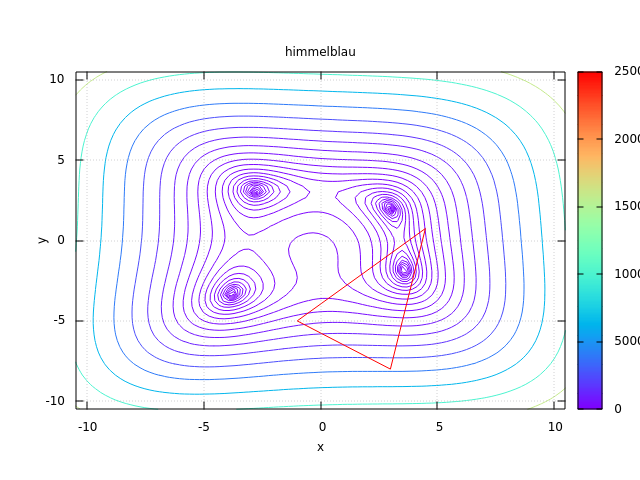
\includegraphics[width=0.7\textwidth]{nelder_mead/2}
    \caption{Unser Simplex nach dem ersten Transformationsschritt}
\end{figure}

Nun berechnen wir den neuen Mittelpunkt und reflektierten Punkt

\begin{eqnarray*}
    M = \frac{B + G}{2} = \binom{1.75}{-2.125}\\
    R = 2M - W = \binom{0.5}{3.75}
\end{eqnarray*}

Nun berechnen wir $f(R) = 106.19141$ und sehen, dass dies Relation $f(B) \leq f(R) \leq f(W)$ erfüllt ist. Wir akzeptieren also
den reflektierten Punkt und ordnen unsere Werte neu.

\begin{eqnarray*}
    B & = & (4.5, \, 0.75)\\
    G & = & (0.5,\,3.75)\\
    W & = & (-1,\,-5)
\end{eqnarray*}

\begin{figure}[H]
    \centering
    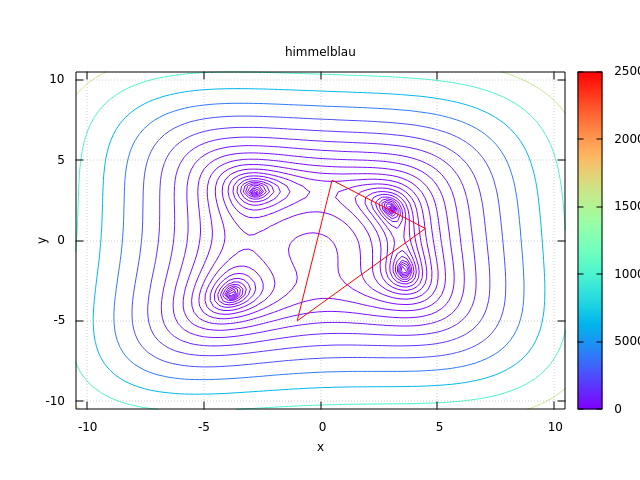
\includegraphics[width=0.7\textwidth]{nelder_mead/3}
    \caption{Unser Simplex nach dem zweiten Transformationsschritt}
\end{figure}

Wir berechnen den neuen Mittelpunkt $M = \binom{2.5}{2.25}$ und den neuen
reflektierten Punkt $R = \binom{6}{9.5}$. $f(R) = 9155.815$, wir erreichen also
keine Verbesserung. Wir berechnen wiederum den inneren kontrahierten Punkt
$C_{2} = \binom{0.75}{-1.375}$ und sehen, dass $f(C_{2}) = 158.53931$, also
eine Verbesserung gegenüber $f(W) = 514$. Wir akzeptieren also $C_{2}$ und
ordnen unsere Punkte neu.

\begin{eqnarray*}
    B & = & (4.5, \, 0.75)\\
    G & = & (0.5,\,3.75)\\
    W & = & (0.75,\,-1.375)
\end{eqnarray*}

\begin{figure}[H]
    \centering
    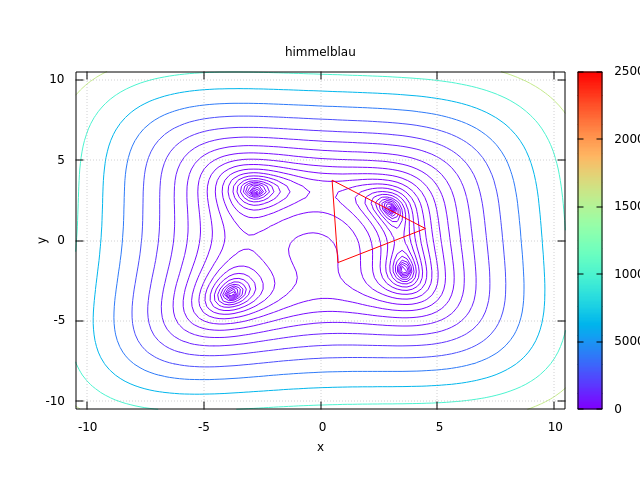
\includegraphics[width=0.7\textwidth]{nelder_mead/4}
    \caption{Nach dem dritten Transformationsschritt}
\end{figure}

Die beiden besten Punkte haben sich nicht geändert, also bleibt auch der
Mittelpunkt gleich. Wir berechnen den reflektierten Punkt als $R =
\binom{4.25}{5.875}$. Da $f(R) = 1176.43384$ haben wir keine Verbesserung
erreicht und sind sogar schlechter als der schlechteste Punkt unseres Simplex',
demnach berechnen wir wiederum den inneren kontrahierten Punkt $C_{2} =
\binom{1.625}{0.4375}$. Der Funktionswert an der Stelle $C_{2}$ ist $89.62574$
und damit besser als $B$. Wir akzeptieren diesen Punkt daher und ordnen unsere
Punkte neu.

\begin{eqnarray*}
    B & = & (1.625,\,0.4375)\\
    G & = & (4.5, \, 0.75)\\
    W & = & (0.5,\,3.75)
\end{eqnarray*}

\begin{figure}[H]
    \centering
    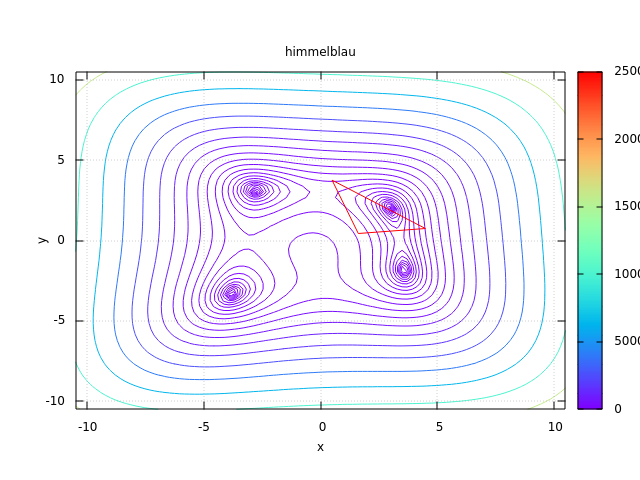
\includegraphics[width=0.7\textwidth]{nelder_mead/5}
    \caption{Nach dem vierten Transformationsschritt}
\end{figure}

Es ist mittlerweile klar, dass wir im Punkt $\binom{3}{2}$ konvergieren werden.
Das beliegende {\tt C++}-Programm konvergierte mit den angegebenen Parametern
in 23 Iterationsschritten. Die weiteren Schritte werden hier mit dem Verweis
auf die Implementierung und die {\tt .gif}-Datei auf der Projektwebseite ausgelassen.


\subsection{Analyse}

Die formale mathematische Analyse des Nelder-Mead-Algorithmus' ist nicht möglich.
Es kann nicht eindeutig bewiesen werden, dass der Algorithmus beim Bearbeiten einer gegebenen
Funktion $f_x$ konvergiert. Die Annahme, dass der Simplex konvergiert, beruht auf zwei
Gegebenheiten:

\begin{itemize}
\item Der Simplex degeneriert nicht während der Laufzeit.
\item Irgendeine Art eines Abstiegskriteriums wird verwendet.
\end{itemize}

Beides ist \emph{nicht} gegeben -- der Simplex kann und wird in einigen Fällen
beinahe degenerieren, sofern die Landschaft der Funktion dies
zulässt.
\footnote{Man betrachte Rosenbrock's Bananenfunktion, in deren Tal der Simplex
    rapide schrumpft und sich somit nur mehr sehr langsam bewegen
kann.} Weiters ist das Abstiegskriterion mehr zufällig -- es ist nicht mathematisch
fundiert wie etwa die Verwendung des negativen Gradienten, der mathematisch beweisbar
immer in die Richtung des steilsten Abstiegs zeigt. \cite{nelder-mead-scholarpedia}

Nichtsdestotrotz ist der Nelder-Mead-Algorithmus ein guter ableitungsfreier
Optimierungsalgorithmus, der zumeist zuverlässig korrekte Resultate liefert.
Tatsächlich gibt es aber eine ganze Familie von Funktionen, für die das Nelder-Mead-Verfahren
immer zu einem Punkt konvergiert, der nicht das Minimum ist\cite{nelder-mead-convergence}.

In vielen naturwissenschaftlichen Bereichen sind Funktionswerte fehlerbehaftet und damit
genaue Lösungen unnötig. In diesen Fällen ist der Nelder-Mead-Algorithmus von großem
Vorteil, da er schnell Ergebnisse liefert die oft bereits ,,gut genug'' sind.
Dazu kommt selbstverständlich die Tatsache, dass der vorliegende Algorithmus anschaulich
und relativ leicht verständlich ist, und viele natürlich mehr inkliniert sind, Methoden
zu verwenden, die sie auch verstehen.

\section{Das Gradientenverfahren}

\subsection{Die Idee und der Zweck des Gradientenverfahren}

Grundsätzlich ist das Gradientenverfahren ein Optimierungsverfahren, welches
das Minimum einer mehrdimensionalen Funktion errechnen. Der Gradient
(${\nabla}f(x,y)$) einer Funktion \(f(x)\) zeigt, aus später gezeigten
\footnote{HIER VERWEIS EINFÜGEN} Gründen, immer in die Richtung des steilsten
Anstiegs, folglich zeigt -${\nabla}f(x,y)$ in die Richtung des stärksten
Abstiegs. Das Gradientenverfahren macht sich dies zunutze und man ``wandert''
eine gewisse Dauer in diese Richtung, wie \textquotedbl{}lange\textquotedbl{}
man in die errechnete Richtung \textquotedbl{}wandert\textquotedbl{} hängt
unter anderem auch von der gewählten Methode ab.

\begin{figure}[H]
    \centering
    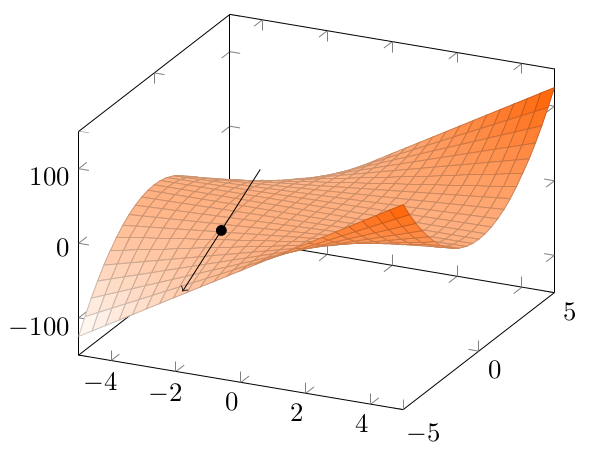
\includegraphics[width=0.7\textwidth]{grad/figure0}
    \caption[Gradientenvektor Beispiel] {Hier zu sehen ist -$\vec{\nabla}f(-2,-2)$ der Funktion $f(x,y)=x*y^2$}
\end{figure}

\subsection{Der Ablauf des Gradientenverfahrens}
\begin{enumerate}
    \item Es wird ein beliebiger Startpunkt $P=(x,y)$ ausgewählt.
    \item Es wird die Ableitung der Funktion $f(x,y)$, also ${\nabla}f(x)$
        gebildet. Sollte dieser Gradient bereits den Wert null haben sind
        wir bereits fertig und haben ein lokales Minimum.
    \item Der Punkt $P$ wird in den Gradienten eingesetzt und der negative
        Wert berechnet, also $-{\nabla}f(x_{P},y_{P})$.
    \item Um eine neuen Punkt $P^{[n+1]}$ zu finden stellen wir nun folgende
        Gleichung auf: $P^{[n+1]} = P^{[n]} + \alpha_{[n]} * s^{[n]}$. Nun
        haben wir die Richtung in die optimiert werden muss gefunden ($s^{[n]}$
        ($=-{\nabla}f(x_{P},y_{P})$)), jetzt muss noch entschieden werden
        wie weit wir in diese Richtung \textquotedbl{}wandern\textquotedbl{}
        ($\alpha^{[n]}$, liegt zwischen $0$ und $1$) (Hinweis: $n$ ist
        die aktuelle Iteration). \\\\ Das kann man einerseits mit Hilfe eines
        fixen Werts machen, andererseits auch mit einer Folge (wie z.B $\frac{1}{\sqrt{n}}$)
        oder einer jedes mal neu errechneten Schrittweite. Zu beachten ist,
        dass die ausgewählte Folge auf jeden Fall divergent sein muss, da
        man sonst bis zu einer maximalen Entfernung ``wandern''
        kann und die Wahrscheinlichkeit groß ist das Optimum nie zu erreichen.
        Sollte man jedes mal einen fixen Wert verliert man zwar den Aufwand
        für die Berechnung der Schrittweite, jedoch ist die Wahrscheinlichkeit
        hoch, dass man viele Iterationen benötigt oder in einer endlosen Schleife
        festhängt. \\\\ Es gibt verschieden Arten wie man die Schrittweite
        berechnen kann, im Folgenden werde ich die Schrittweitenbestimmung
        nach Armijo erklären. Dieses Verfahren ist eines der sogenannten \textquotedbl{}line-search\textquotedbl{}
        Verfahren, das von mir gezeigte ist jedoch kein exaktes line-search
        Verfahren sondern lediglich eine einfache Heuristik. \\\\ \textbf{Die Armijo-Bedingung:}
        $\varphi(\alpha) \leq \varphi(0) + c * \alpha^{[n]} * \varphi(0)'$.
        \\\\ Wobei $c$ eine Konstante zwischen null und eins ist und dazu
        dient das die Bedingung nicht zu restriktiv ist, $\varphi(\alpha) = f(P^{[n]} + \alpha^{[n]}s^{[n]})$
        und $\varphi(0)' = {\nabla}f(P^{n}) * s^{[n]}$
    \item Für den Anfang wird $\alpha=1$ gewählt und errechnet ob die Armijo-Bedingung
        erfüllt ist - sollte sie erfüllt sein haben wir ein passende $\alpha$
        gefunden, wenn nicht wird $\alpha$ mit einem $\beta$, welches ebenfalls
        zwischen null und eins liegt, multipliziert und wieder geprüft ob
        die Ungleichung erfüllt ist. (Hinweis: In der Praxis liefern die Werte
        $c = 0.01$ und $\beta = 0.9$ häufig gute Ergebnisse.
        \footnote{\href{https://www.unibw.de/lrt1/gerdts/lehre/lpnlp/lp-nlp.pdf}{https://www.unibw.de/lrt1/gerdts/lehre/lpnlp/lp-nlp.pdf}}
    \item Wenn man einen neuen Punkt gefunden hat wird bei Punkt 3 fortgesetzt.
        Da es oft einen großen Rechenaufwand erfordert das genaue Minimum
        zu finden wird das Verfahren meist beendet wenn der Gradient einen
        akzeptablen Wert erreicht hat (So kann man als Abbruchbedingung z.B.
        die stärke des Anstiegs in einem Punkt (also den Betrag des Gradienten)
        nehmen).
\end{enumerate}

\subsection{Beispiele}
\subsubsection{Beispiel 1}
Zu minimierende Funktion: $f(x,y)=y^4+2x^2-3xy+1$, als Abbruchbedingung wählen
wir $|{\nabla}f(x,y)| \leq 0.3$.

\begin{figure}[H]
    \centering
    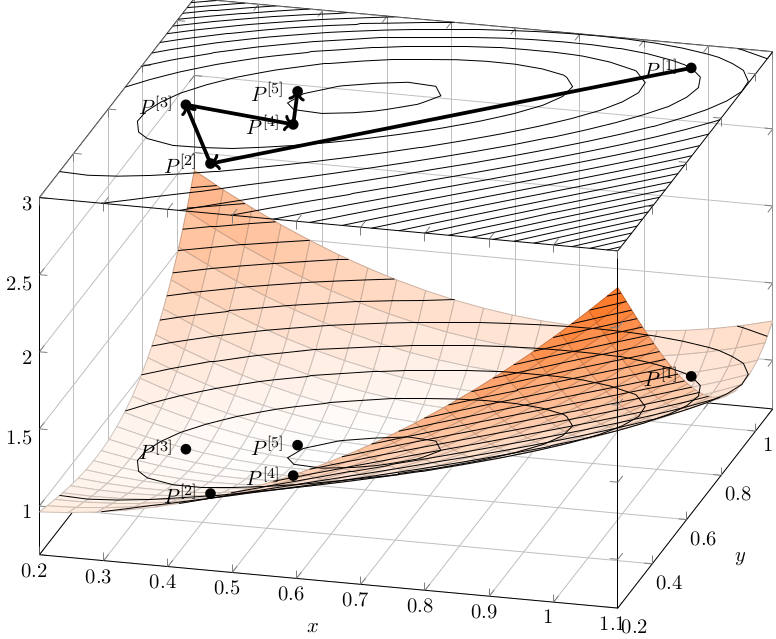
\includegraphics[width=0.7\textwidth]{grad/figure1}
    \caption{Beispiel 1. Zusätzlich sind hier die Höhenschichtlinien eingezeichnet.}
    \label{bsp1}
\end{figure}
Wie man in Abbildung~\ref{bsp1} sieht, nähert man sich schrittweise dem
Minimum an.

\begin{figure}[H]
    \centering
    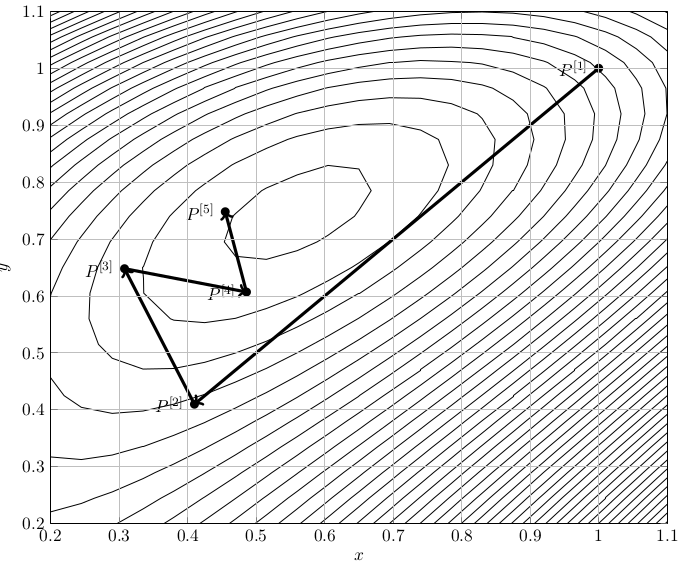
\includegraphics[width=0.7\textwidth]{grad/figure2}
    \caption{Die Höhenschichtlinien genauer gezeigt.}
\end{figure}

\begin{enumerate}
	\item
	Startpunkt $P=(1,1)$
	\item
	Ableitung: ${\nabla}f(x,y)=
	\left( \begin{array}{c}
	4x-3y \\
	4y^3-3x
	\end{array} \right)
	$($\rightarrow$ Der Gradient)
	\item
	$-{\nabla}f(1,1) =
	\left( \begin{array}{c}
	-4+3 \\
	-4+3
	\end{array} \right)
	=
	\left( \begin{array}{c}
	-1 \\
	-1
	\end{array} \right)
	$ ($\rightarrow$ Richtung des stärksten Abstiegs)
	\item
	Die Armijo-Bedingung (mit $\alpha = 1$, $c = 0.1$ und $\beta = 0.9$):\\
	$f( \left( \begin{array}{c} 1 \\ 1 \end{array} \right) + 1 * \left( \begin{array}{c} -1 \\ -1 \end{array} \right)) \leq f(\left( \begin{array}{c} 1 \\ 1 \end{array} \right)) + 0.1 * 1 *  \left( \begin{array}{c} 1 \\ 1 \end{array} \right) * \left( \begin{array}{c} -1 \\ -1 \end{array} \right)$ \\
	$= 1 \leq 0.8$ \\
	$\rightarrow \alpha^{[2]} = \alpha^{[1]} * \beta = 0.9$ \\

	$f( \left( \begin{array}{c} 1 \\ 1 \end{array} \right) + 0.9 * \left( \begin{array}{c} -1 \\ -1 \end{array} \right)) \leq f(\left( \begin{array}{c} 1 \\ 1 \end{array} \right)) + 0.1 * 0.9 *  \left( \begin{array}{c} 1 \\ 1 \end{array} \right) * \left( \begin{array}{c} -1 \\ -1 \end{array} \right)$ \\
	$= 0.99 \leq 0.82$ \\
	$\rightarrow \alpha^{[3]} = \alpha^{[2]} * \beta = 0.81$ \\

	$f( \left( \begin{array}{c} 1 \\ 1 \end{array} \right) + 0.81 * \left( \begin{array}{c} -1 \\ -1 \end{array} \right)) \leq f(\left( \begin{array}{c} 1 \\ 1 \end{array} \right)) + 0.1 * 0.81 *  \left( \begin{array}{c} 1 \\ 1 \end{array} \right) * \left( \begin{array}{c} -1 \\ -1 \end{array} \right)$ \\
	$= 0.965 \leq 0.838$ \\
	$\rightarrow \alpha^{[4]} = \alpha^{[3]} * \beta = 0.729$ \\

	$f( \left( \begin{array}{c} 1 \\ 1 \end{array} \right) + 0.729 * \left( \begin{array}{c} -1 \\ -1 \end{array} \right)) \leq f(\left( \begin{array}{c} 1 \\ 1 \end{array} \right)) + 0.1 * 0.729 *  \left( \begin{array}{c} 1 \\ 1 \end{array} \right) * \left( \begin{array}{c} -1 \\ -1 \end{array} \right)$ \\
	$= 0.932 \leq 0.854$ \\
	$\rightarrow \alpha^{[5]} = \alpha^{[4]} * \beta = 0.656$ \\

    $f( \left( \begin{array}{c} 1 \\ 1 \end{array} \right) + 0.656 * \left( \begin{array}{c} -1 \\ -1 \end{array} \right)) \leq f(\left( \begin{array}{c} 1 \\ 1 \end{array} \right)) + 0.1 * 0.656 *  \left( \begin{array}{c} 1 \\ 1 \end{array} \right) * \left( \begin{array}{c} -1 \\ -1 \end{array} \right)$ \\
    $= 0.896 \leq 0.869$ \\
    $\rightarrow \alpha^{[6]} = \alpha^{[5]} * \beta = 0,59$ \\

    $f( \left( \begin{array}{c} 1 \\ 1 \end{array} \right) + 0,59 * \left( \begin{array}{c} -1 \\ -1 \end{array} \right)) \leq f(\left( \begin{array}{c} 1 \\ 1 \end{array} \right)) + 0.1 * 0,59 *  \left( \begin{array}{c} 1 \\ 1 \end{array} \right) * \left( \begin{array}{c} -1 \\ -1 \end{array} \right)$ \\
    $= 0.86 \leq 0.882$ \\
    Nun haben wir ein passendes $\alpha$ gefunden und können zum nächsten Punkt wandern.

    \begin{figure}[H]
        \centering
        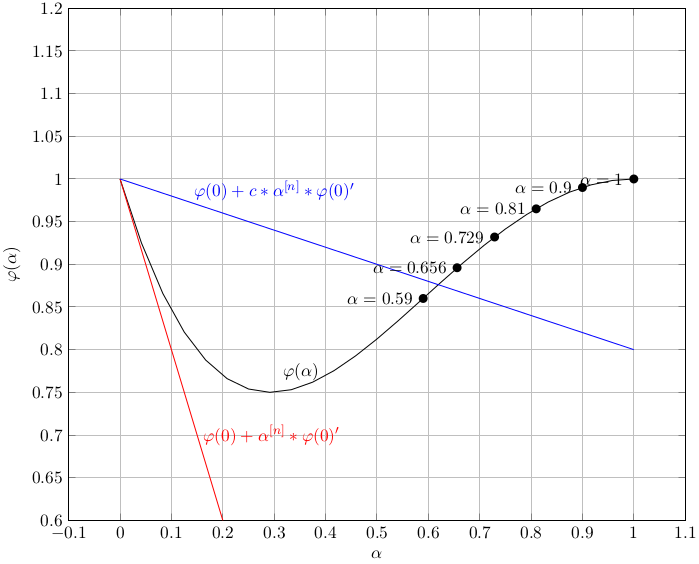
\includegraphics[width=0.7\textwidth]{grad/figure3}
        \caption[Die Armijo-Bedingung] {Hier sieht man die Funktion $\varphi(\alpha)=(1-\alpha)^4+2*(1-\alpha)^2-3*(1-\alpha)*(1-\alpha)+1)$, sie ist sozusagen ein Durchschnitt durch die bei Beispiel 1 gegebene Funktion. Diese Funktion wird erzeugt, wenn man vom Punkt $P^{[1]}=(1,1)$ in Richtung des Gradienten wandert. Die blaue Gerade zeigt die Armijo-Bedingung bei $c=0.1$, die rote bei $c=1$ bzw. ohne c.}
    \end{figure}

    \item
    $P^{[2]} = \left( \begin{array}{c} 1 \\ 1 \end{array} \right) + 0,59 * \left( \begin{array}{c} -1 \\ -1 \end{array} \right) = \left( \begin{array}{c} 0.41 \\ 0.41 \end{array} \right)$
    \item
    $-{\nabla}f(0.41,0.41) = \left( \begin{array}{c} -0.41 \\ 0.95 \end{array} \right)$, \\
	$|{\nabla}f(0.41,0.41)| = \sqrt{0.41^2+0.95^2} = 1.071$
	\item
	Die Armijo-Bedingung (mit $\alpha = 1$, $c = 0.1$ und $\beta = 0.5$):\\
	$f( \left( \begin{array}{c} 0.41 \\ 0.41 \end{array} \right) + 1 * \left( \begin{array}{c} -0.41 \\ 0.95 \end{array} \right)) \leq f(\left( \begin{array}{c} 0.41 \\ 0.41 \end{array} \right)) + 0.1 * 1 *  \left( \begin{array}{c} -0.41 \\ 0.95 \end{array} \right) * \left( \begin{array}{c} 0.41 \\ -0.95 \end{array} \right)$ \\
	$= 4.421 \leq 0.753$
	$\rightarrow \alpha^{[2]} = \alpha^{[1]} * \beta = 0.5$ \\
	$\rightarrow = 1.153 \leq 0.807$
	$\rightarrow \alpha^{[3]} = \alpha^{[2]} * \beta = 0.25$ \\
	$\rightarrow = 0.768 \leq 0.833$
	\item
	$P^{[3]} = \left( \begin{array}{c} 0.41 \\ 0.41 \end{array} \right) + 0.25 * \left( \begin{array}{c} -0.41 \\ 0.95 \end{array} \right) = \left( \begin{array}{c} 0.308 \\ 0.648 \end{array} \right)$
	\item
	$-{\nabla}f(0.308,0.648) = \left( \begin{array}{c} 0.712 \\ -0.164 \end{array} \right)$, \\
	$|{\nabla}f(0.308,0.648)| = \sqrt{0.712^2+0.164^2} = 0.534$
	\item
	Die Armijo-Bedingung (mit $\alpha = 1$, $c = 0.1$ und $\beta = 0.5$):\\
	$f( \left( \begin{array}{c} 0.308 \\ 0.648 \end{array} \right) + 1 * \left( \begin{array}{c} 0.712 \\ -0.164 \end{array} \right)) \leq f(\left( \begin{array}{c} 0.308 \\ 0.648 \end{array} \right)) + 0.1 * 1 *  \left( \begin{array}{c} 0.712 \\ -0.164 \end{array} \right) * \left( \begin{array}{c} -0.712 \\ 0.164 \end{array} \right)$ \\
	$= 1.655 \leq 0.714$
	$\rightarrow \alpha^{[2]} = \alpha^{[1]} * \beta = 0.5$ \\
	$\rightarrow = 0.857 \leq 0.741$
	$\rightarrow \alpha^{[3]} = \alpha^{[2]} * \beta = 0.25$ \\
	$\rightarrow = 0.723 \leq 0.754$
	\item
	$P^{[4]} = \left( \begin{array}{c} 0.308 \\ 0.648 \end{array} \right) + 0.25 * \left( \begin{array}{c} 0.712 \\ -0.164 \end{array} \right) = \left( \begin{array}{c} 0.486 \\ 0.607 \end{array} \right)$
	\item
	$-{\nabla}f(0.486,0.607) = \left( \begin{array}{c} -0.123 \\ 0.563. \end{array} \right)$, \\
	$|{\nabla}f(0.486,0.607)| = \sqrt{0.123^2+0.563^2} = 0.332$
	\item
	Die Armijo-Bedingung (mit $\alpha = 1$, $c = 0.1$ und $\beta = 0.5$):\\
	$f( \left( \begin{array}{c} 0.486 \\ 0.607 \end{array} \right) + 1 * \left( \begin{array}{c} -0.123 \\ 0.563 \end{array} \right)) \leq f(\left( \begin{array}{c} 0.486 \\ 0.607 \end{array} \right)) + 0.1 * 1 *  \left( \begin{array}{c} -0.123 \\ 0.563 \end{array} \right) * \left( \begin{array}{c} 0.123 \\ -0.563 \end{array} \right)$ \\
	$= 1.863 \leq 0.689$
	$\rightarrow \alpha^{[2]} = \alpha^{[1]} * \beta = 0.5$ \\
	$\rightarrow = 0.852 \leq 0.707$
	$\rightarrow \alpha^{[3]} = \alpha^{[2]} * \beta = 0.25$ \\
	$\rightarrow = 0.706 \leq 0.715$
	\item
	$P^{[5]} = \left( \begin{array}{c} 0.486 \\ 0.607 \end{array} \right) + 0.25 * \left( \begin{array}{c} -0.123 \\ 0.563 \end{array} \right) = \left( \begin{array}{c} 0.455 \\ 0.748 \end{array} \right)$
    \item
	$-{\nabla}f(0.455,0.748) = \left( \begin{array}{c} 0.424 \\ -0.309. \end{array} \right)$, \\
	$|{\nabla}f(0.455,0.748)| = \sqrt{0.424^2+0.309^2} = 0.275$ \\
	Die Abbruchbedingung ist erfüllt und somit ist ein Punkt, welcher nahe genug am Optimum liegt gefunden.


\end{enumerate}


\section{Die Koordinatenabstiegsmethode}

\subsection{Einführung}

Bei der Koordinatenabstiegsmethode wird bei jedem Schritt eine Koordinate
i gewählt, nach der man optimiert. Es wird bei einem beliebigen Startpunkt
begonnen und in jedem Iterationsschritt setzt man alle Koordinaten
des aktuellen Punktes in die Funktion ein , nur die Koordinate , nach
der man minimieren will , behält man als Variable bei.

Es wird immer in Richtung einer Achse minimiert und die Stelle , an
der das Minimum ist , als neue Koordinate beibehalten und so gelangt
man mit einer Anzahl an Iterationen zum Minimum der Funktion.

\begin{figure}[H]
    \centering
    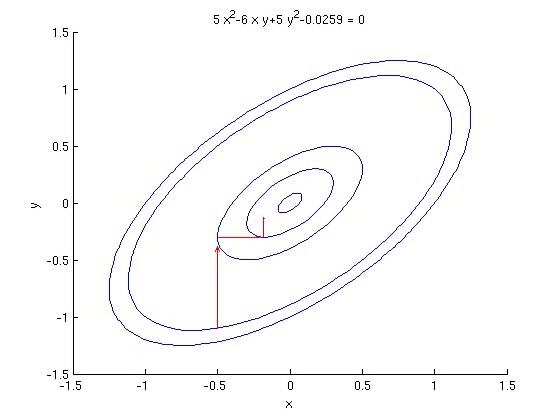
\includegraphics[width=0.7\textwidth]{coord_desc/Coordinate_descent}
    \caption{Die Koordinatenabstiegsmethode}
\end{figure}

~\\
Wenn zum Beispiel die Funktion $f(x,y)=2x^{2}+2xy+1.5y^{2}$ und der
Startpunkt $P=(1,\,1)$ gegeben ist, so muss man, wenn entlang der
$x$-Achse minimiert werden soll folgendes eingesetzt werden:

\begin{eqnarray*}
    x & = & 1+1d\\
    y & = & 1+0d
\end{eqnarray*}


Soll entlang der $y$-Achse optimiert werden, so muss folgendes eingesetzt
werden:

\begin{eqnarray*}
    x & = & 1+0d\\
    y & = & 1+1d
\end{eqnarray*}



\subsection{Beispiel}

Wir möchten die Funktion $f(x,y)=2x^{2}+2xy+1.5y^{2}$ optimieren
und wählen den Startpunkt $P_{0}=(1,\,1)$. Wir minimieren zuerst
entlang der $x$-Achse und setzen ein

\begin{eqnarray*}
    f(d) & = & 2(1+d)^{2}+2(1+d)+1.5\\
    & = & 2d^{2}+6d+5.5
\end{eqnarray*}

Diese soeben erhaltene Funktion müssen wir nun noch minimieren.

\begin{eqnarray*}
    f'(d) & = & 4d+6\\
    4d+6 & = & 0\\
    d & = & \frac{3}{2}
\end{eqnarray*}


Setzen wir dies in die Gleichung für die $x$-Koordinate ein und verwenden
die alte $y$-Koordinate erhalten wir den neuen Punkt $P_{1}=(-\frac{1}{2},\,1)$.
Nun minimieren wir nach $y$, wir setzen also ein:

\begin{eqnarray*}
    x & = & -\frac{1}{2}+0d\\
    y & = & 1+1d
\end{eqnarray*}


und erhalten

\[
    f(d)=1.5d^{2}-d+6
\]

Dies minimieren wir wiederum und erhalten die neue $y$-Koordinate
$\frac{1}{3}$. Damit haben wir den neuen Punkt $(-\frac{1}{2},\:\frac{1}{3}$).
Dieser Vorgang wird wiederholt, bis sich die errechneten Werte nurnoch
marginal unterscheiden. Danach wird abgebrochen.


\subsection{Problemfälle}
\begin{quotation}
    \noindent Zeigen Sie, dass die Koordinatenabstiegsmethode für die stetige Funktion
    \[
        f(x,\,y)=
        \begin{cases}
            (x+y-5)^{2}+(x-y-2)^{2} & falls\;x\le y\\
            (x+y-5)^{2}+(x-y+2)^{2} & sonst
        \end{cases}
    \]
    beginnend beim Startpunkt $(0,\,0)$ nicht funktioniert.
\end{quotation}
Wir setzen ein:

\begin{eqnarray*}
    x & = & d\\
    y & = & 0
\end{eqnarray*}
und erhalten die Funktion

\begin{eqnarray*}
    f(d) & = & (d-5)^{2}+(d-2)^{2}\\
    & = & 2d^{2}-14d+29
\end{eqnarray*}
welche ein Minimum an der Stelle $d=\frac{7}{2}$ hat. Dies fortgesetzt
für $y$ erhalten wir den neuen Punkt $P=(\frac{7}{2},\,\frac{7}{2})$.
Bei weiteren Iterationen merken wir, dass $d$ immer 0 beträgt \textendash{}
was bedeutet, dass sich der Punkt nicht weiterbewegt. Wir sitzen auf
einem lokalen Minimum fest. Führen wir das mit dem anderen Zweig der
Funktion ebenfalls durch, so sehen wir das gleiche Problem.

\bibliography{ops}
\bibliographystyle{unsrt}
\end{document}
